\section{Experimental results}
In this latter analysis, we did not care about the validation of the model: the company's experience guaranteed the correctness of the model itself. On the contrary, our goal was to study how the result of the previous model affected the final measure of the diameter, and how the same is influenced by the position of the three points on the wheel. \\

The main problem encountered in this set of tests, was due to the lack of availability of a complete \acs{WPMS} to perform acquisitions of real rolling points of the \textit{DIMA}. The only system we could use was one under development, and incomplete. Furthermore, it was also bad calibrated, so the performed measures of the diameter was more or less $40 \, mm$ bigger than the nominal size of the target. Thus, was impossible for us to make any comparison with real data.

Despite that, \textsc{Matlab} allowed us to simulate a plausible scenario, in which three laser was involved, and the rolling points was obtained as the intersection between the laser line and a circumference comparable with the wheel. In Figure \ref{fig:diam:virtual} is shown an example of a simulation. In tests described bellow, we tried to generate real scenario to determine points that could be comparable with sets of real data.
  \begin{figure}[t!]
    \centering
    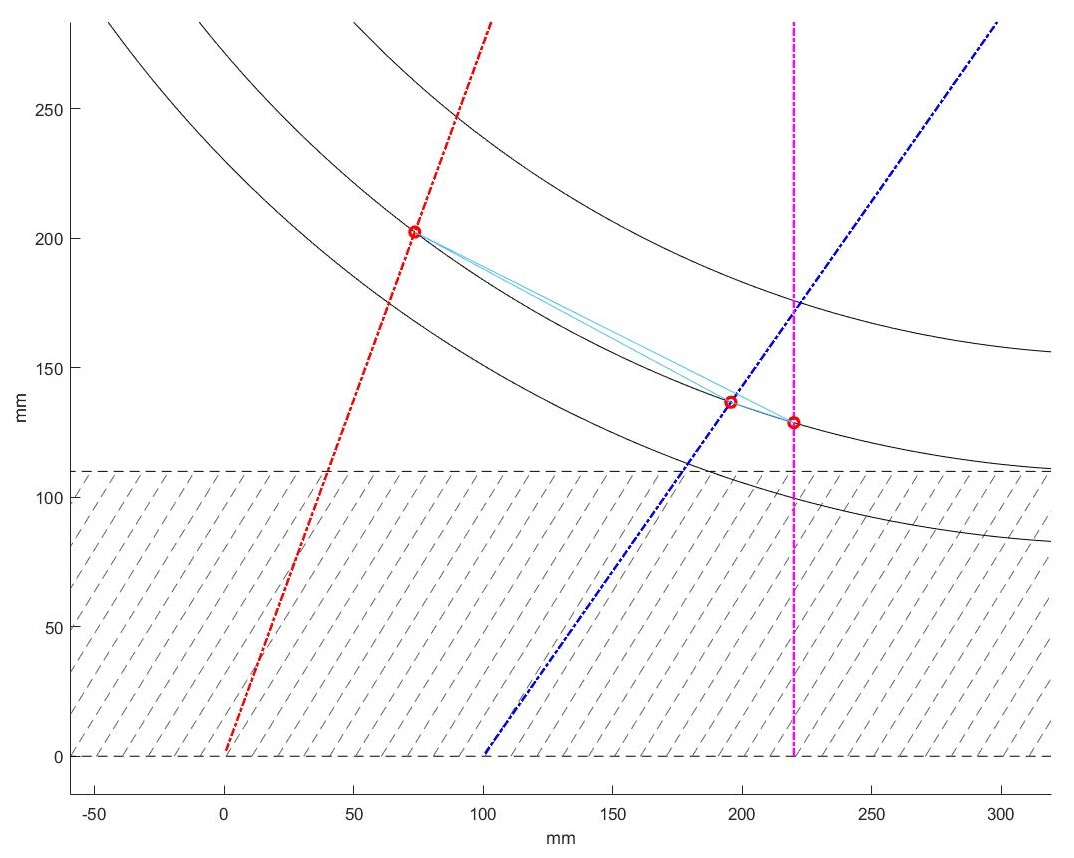
\includegraphics[width=0.75\textwidth]{./images/diameter/virtual.jpg}
    \caption{Example of the simulation used to detect the three rolling points to estimate the diameter of the wheel. The black dotted lines are the rail, while the coloured ones are the laser beams.}
    \label{fig:diam:virtual}
  \end{figure}

\subsection{Effects of points' positions} %%%%%%%%%%%%%%%%%%%%%%%%%%%%%%%%%%%%%%%%%%%%%%%
The first experiments was focus on study the variation of the error with respect to the location of the reference points in the circle. To do that, we analysed two different type of situations:
  \begin{itemize}
    \item in the first one, we moved the wheel in a reasonable range, maintaining the configuration of the acquisition system fixed;
    \item in the second one, we change the positions of the projectors one by one, keeping the others fixed, in order to look for some relations of interest between the configuration of the system and the computed error.
  \end{itemize}

In Figure \ref{fig:diam:dists} we reported the distribution of the errors, obtained with three different setups, moving the wheel along the virtual rail. The first thing we can see, is that these distributions were not linear. Thinking a while, it is easy to understand why: the motion of the points of a circumference, that moves with pure round motion, is a cycloid. So, the relationship between two points determined by the same laser at different times, will have to take into account this quadratic trend. Furthermore, we have to consider that the first order derivative of the Equation \ref{eq:diam:erone} is characterized by the presence of several sine and cosine factors, which prohibit linear distributions. \\
By improving our analysis, we have tried to determine what conditions reduce the final error, and which ones increase it. Initially, we decided to focus on the Distribution \ref{fig:diam:dists1}, because of the presence of a (maybe global) minimum. In Figure \ref{fig:diam:scenarios} we shown the best and the worst scenarios, accordingly with the error. Concerning the worst case, we can notice that a two points was very close to each other, while the third one is far with respect to the others. Looking at all the motion of the wheel, we observed that the error increased as the two points approached. Opposite considerations can be made in the best case: the error decreases as the reciprocal points distance increases. All these consideration suggested us that probably the error was minimum when the points are equally distributed along an arc. Same considerations was reached analysing the scenarios for Distributions \ref{fig:diam:dists2} and \ref{fig:diam:dists3}. Unfortunately, the collected data did not help us. All the attempts made to find a mathematical relation between the location of the points, and the error, failed. \\

Thus, we changed our approach. The great number of parameters we had to consider (the angles of the lasers, their distances from the origin of the reference system, and the length of the $y_i$ vectors) suggested us to simplify the problem. So, we decided to change only one parameter per times, and try to determine the effect of the variation in the final result. Because of the lengths of the vectors $y_i$ strictly depend by the angles $\theta_i$ and by the offsets $H_i$, we decided to ignore them and to focus only in the last parameters. In Figure \ref{fig:diam:hs} we reported the graphical results obtained moving one projector with respect to the others. In this case, we can see how the error decreases increasing the distances between the projectors: differently from the previous scenarios, this is due to the increasing in the length of the arc involved by the three points. However, as we can see from the Figure \ref{fig:diam:hs} (bottom)  the matter is not that simple. It seems that the distribution could be a discontinuous function. The only thing that, in our opinion, may had influence the result, is the angle of the projector with respect of the rail (that is $90\degree$). Many attempt was made to understand how the angle influences the error, but no
  \clearpage
  \begin{figure}[t!]
    \centering
    \begin{minipage}[c]{0.9\textwidth}
      \centering
      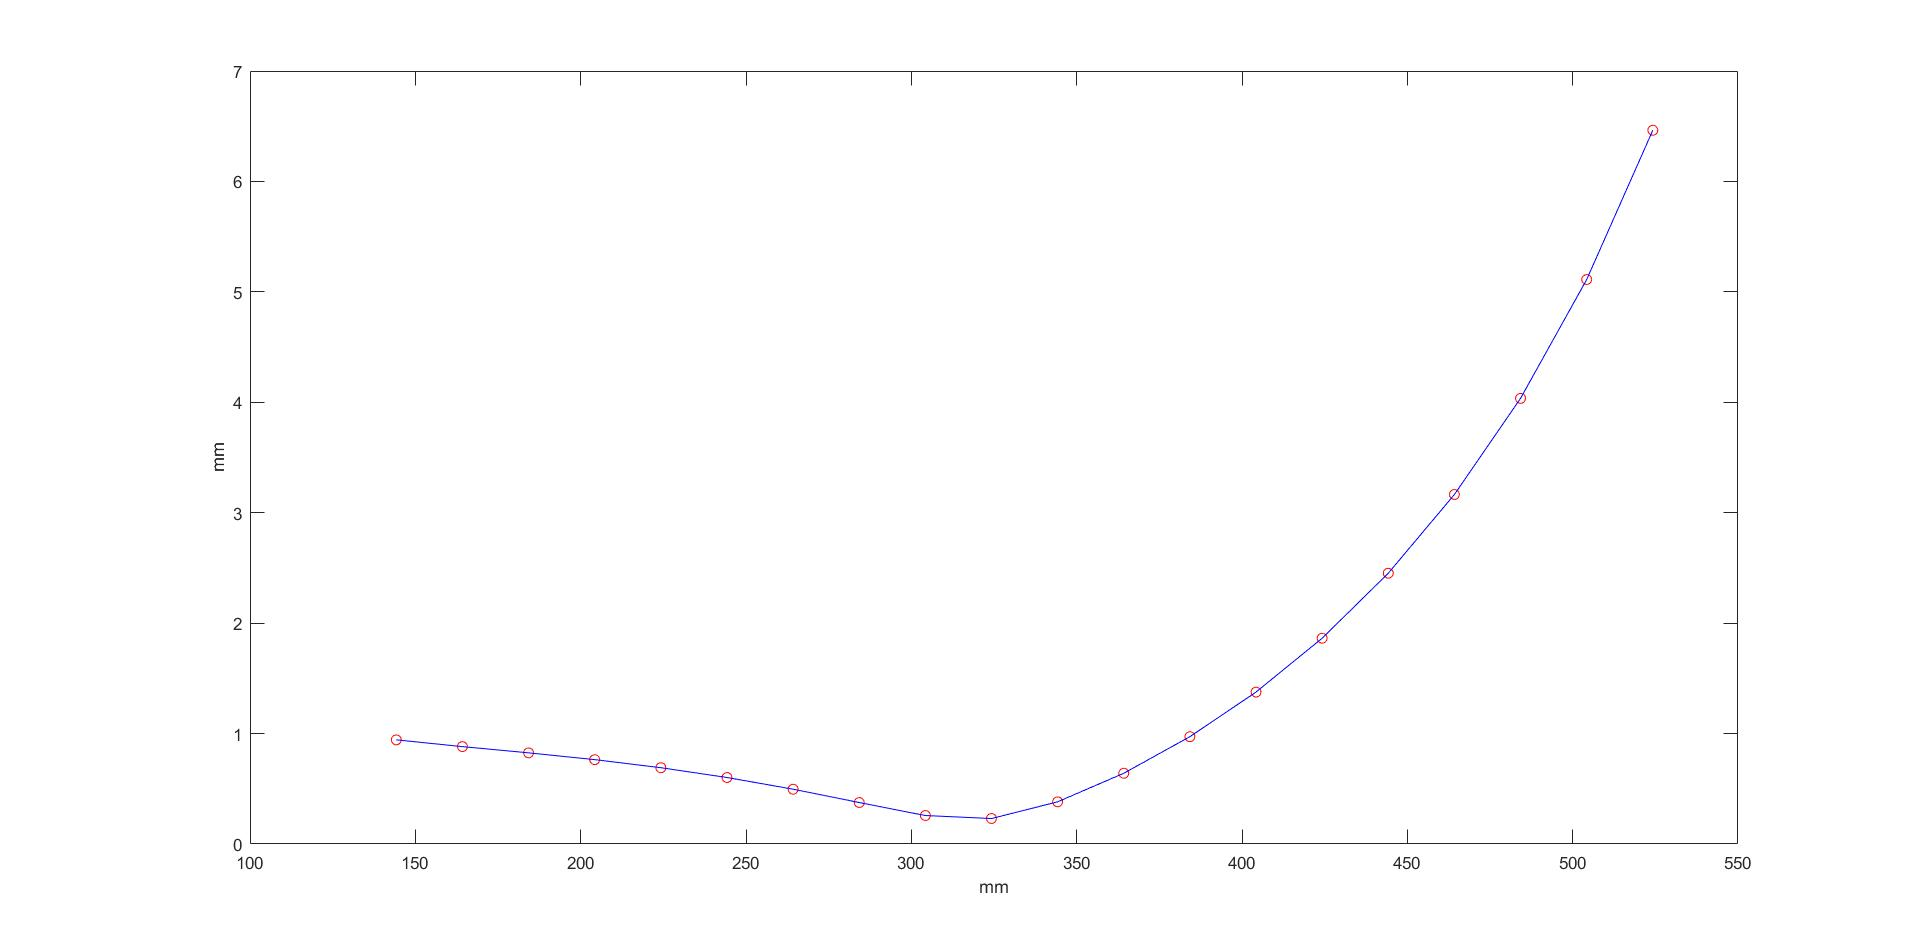
\includegraphics[width=\textwidth]{./images/diameter/distrib1.jpg}
      \subcaption{Distribution \#1}
      \label{fig:diam:dists1}
    \end{minipage}
    \vfill
    \begin{minipage}[c]{0.9\textwidth}
      \centering
      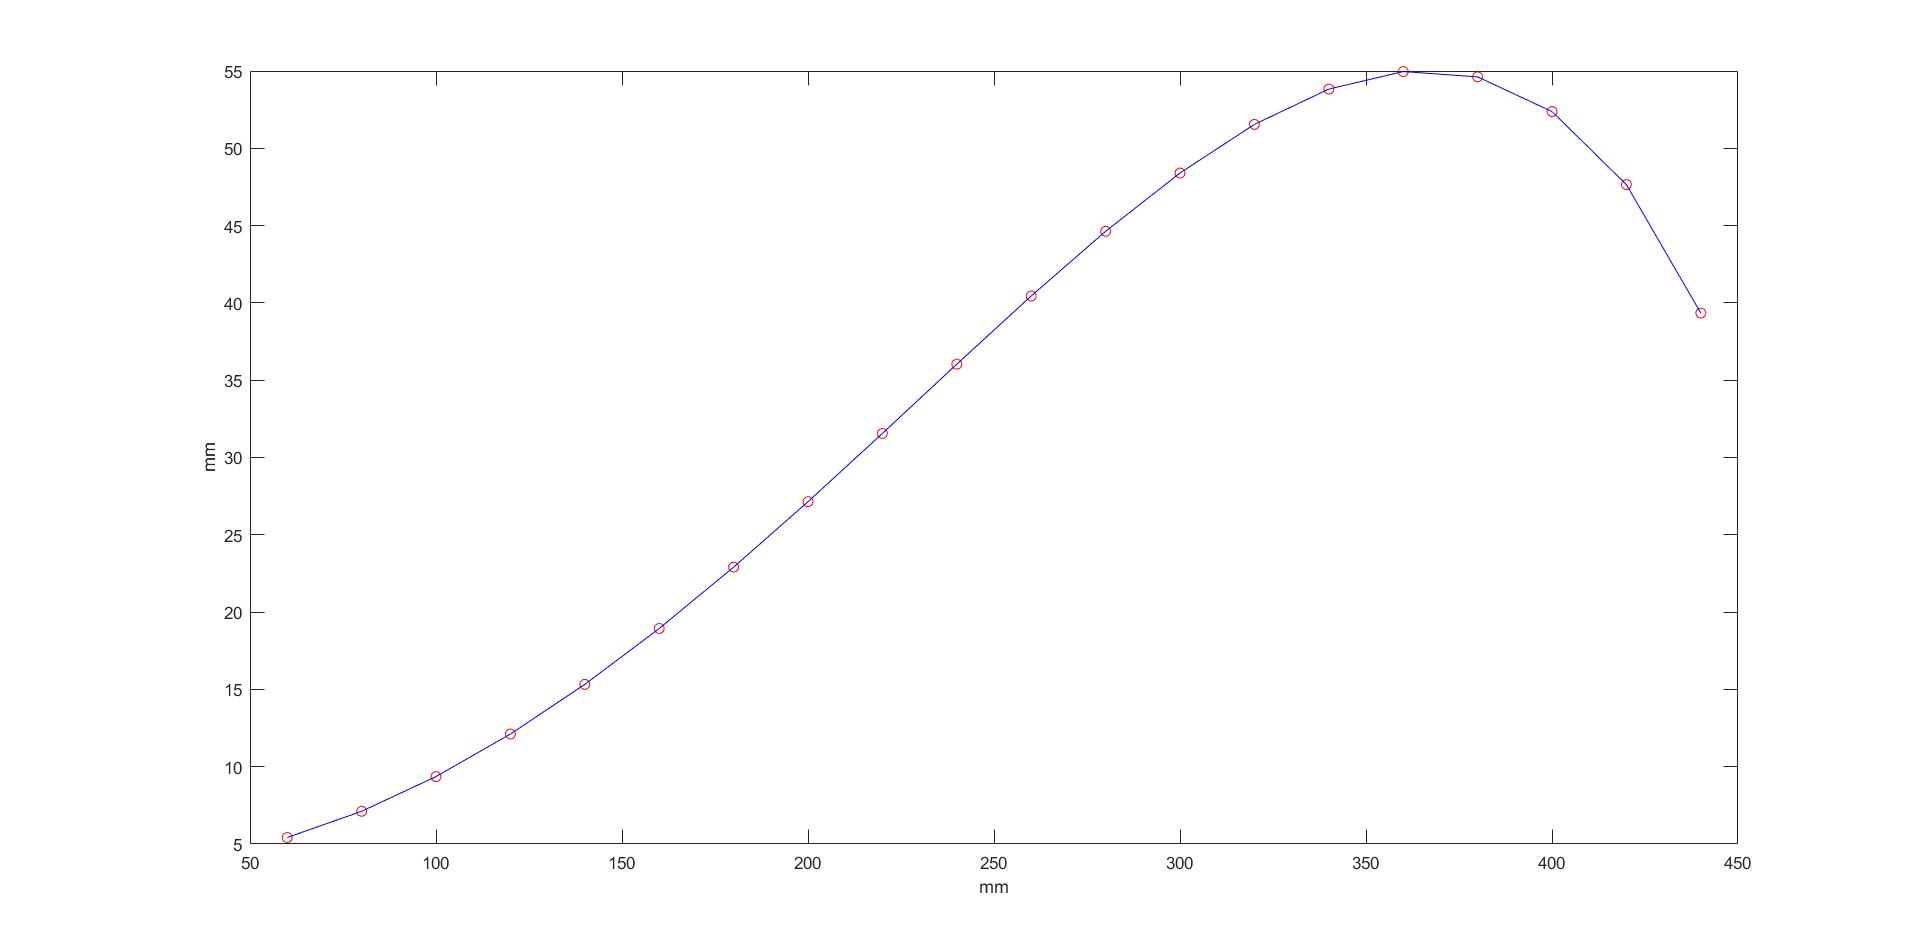
\includegraphics[width=\textwidth]{./images/diameter/distrib2.jpg}
      \subcaption{Distribution \#2}
      \label{fig:diam:dists2}
    \end{minipage}
    \vfill
    \begin{minipage}[c]{0.9\textwidth}
      \centering
      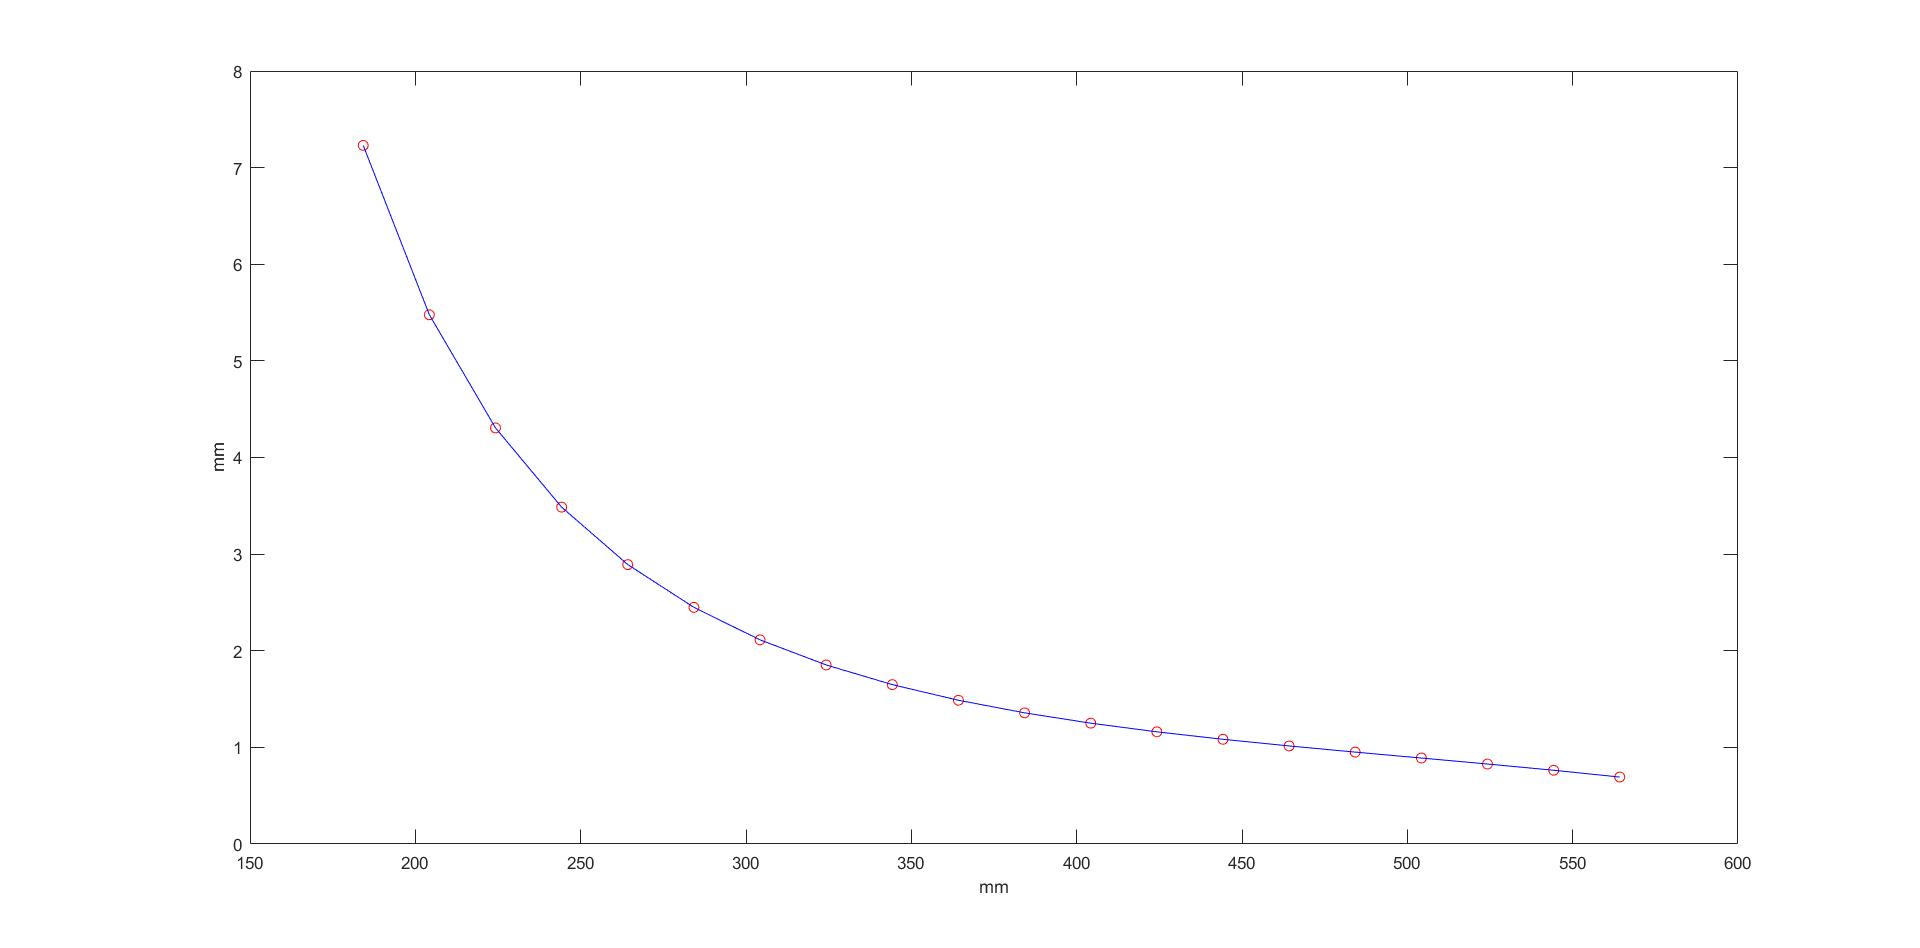
\includegraphics[width=\textwidth]{./images/diameter/distrib3.jpg}
      \subcaption{Distribution \#3}
      \label{fig:diam:dists3}
    \end{minipage}
    
    \caption{Examples of distributions of the final error varying the position of the wheel with respect to the systems.}
    \label{fig:diam:dists}
  \end{figure}
\clearpage %%%%%%%%%%%%%%%%%%%%%%%%%%%%%%%%%%%%%%%%%%%%%%%%%%%%%%%%%%%%%%%%%%%%%%%%%%%%%%%%%%
  \begin{figure}[t!]
    \centering
    \begin{minipage}[c]{\textwidth}
      \centering
      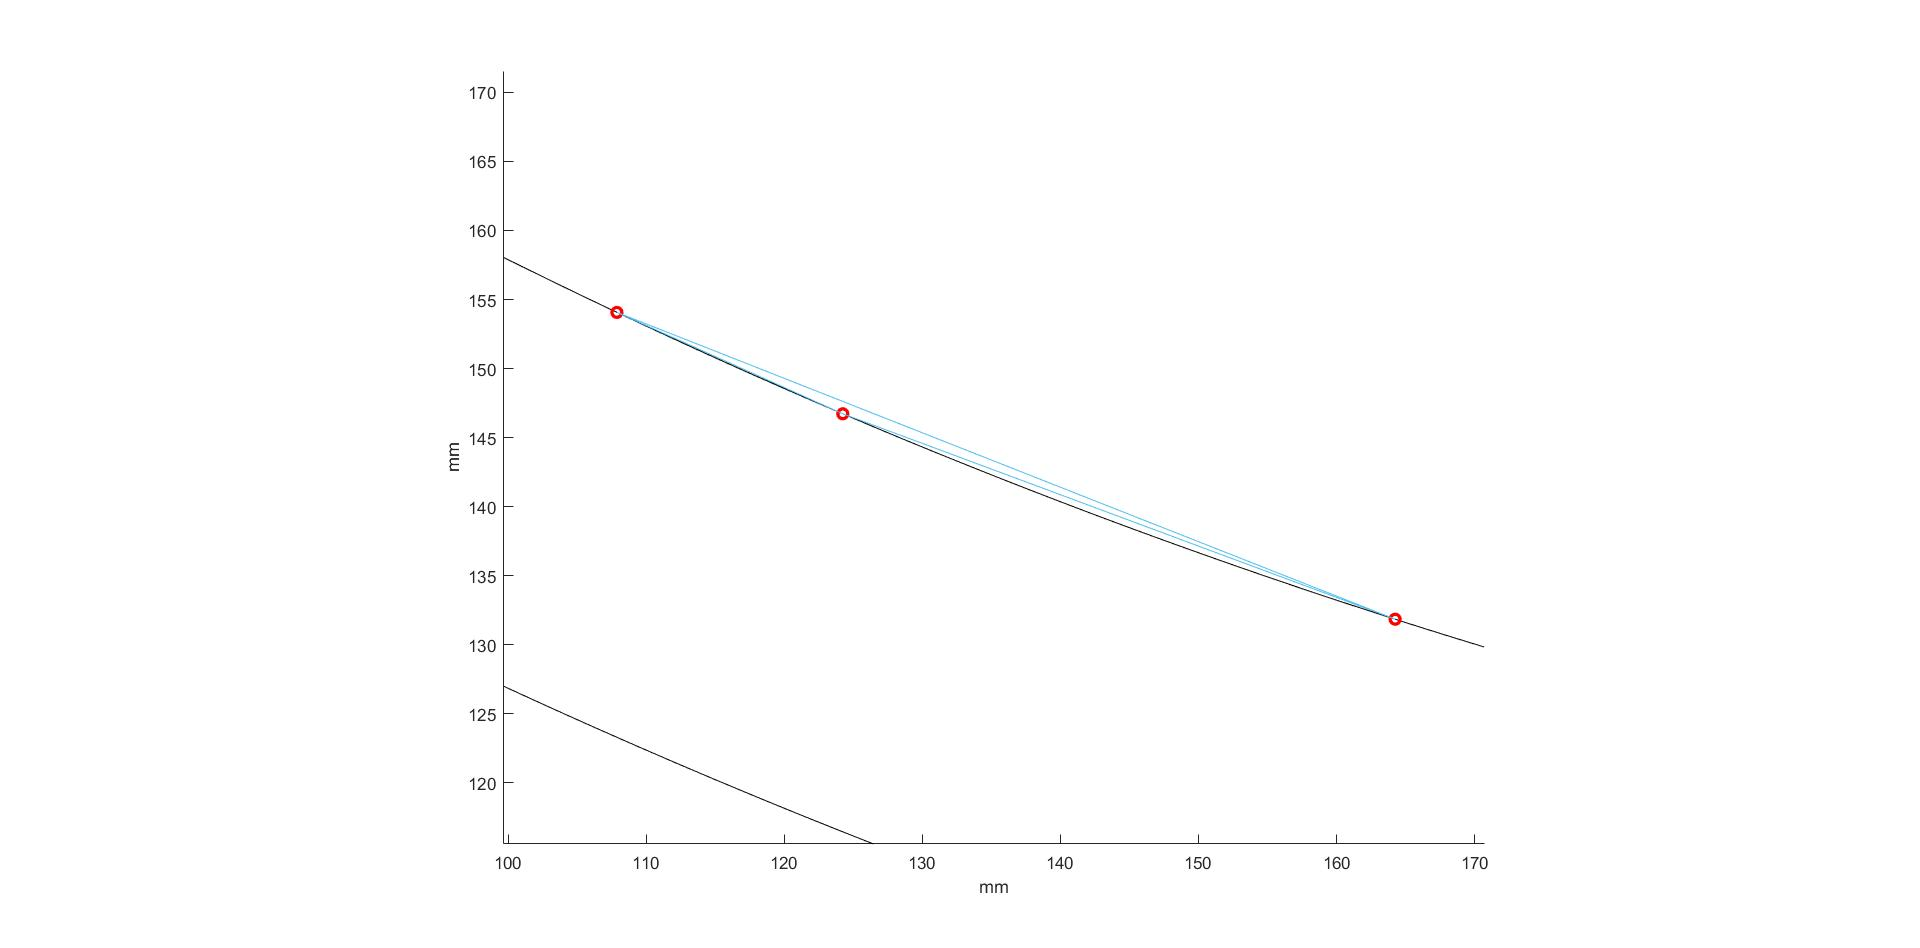
\includegraphics[width=\textwidth]{./images/diameter/c1_better.jpg}
    \end{minipage}
    \vfill
    \begin{minipage}[c]{\textwidth}
      \centering
      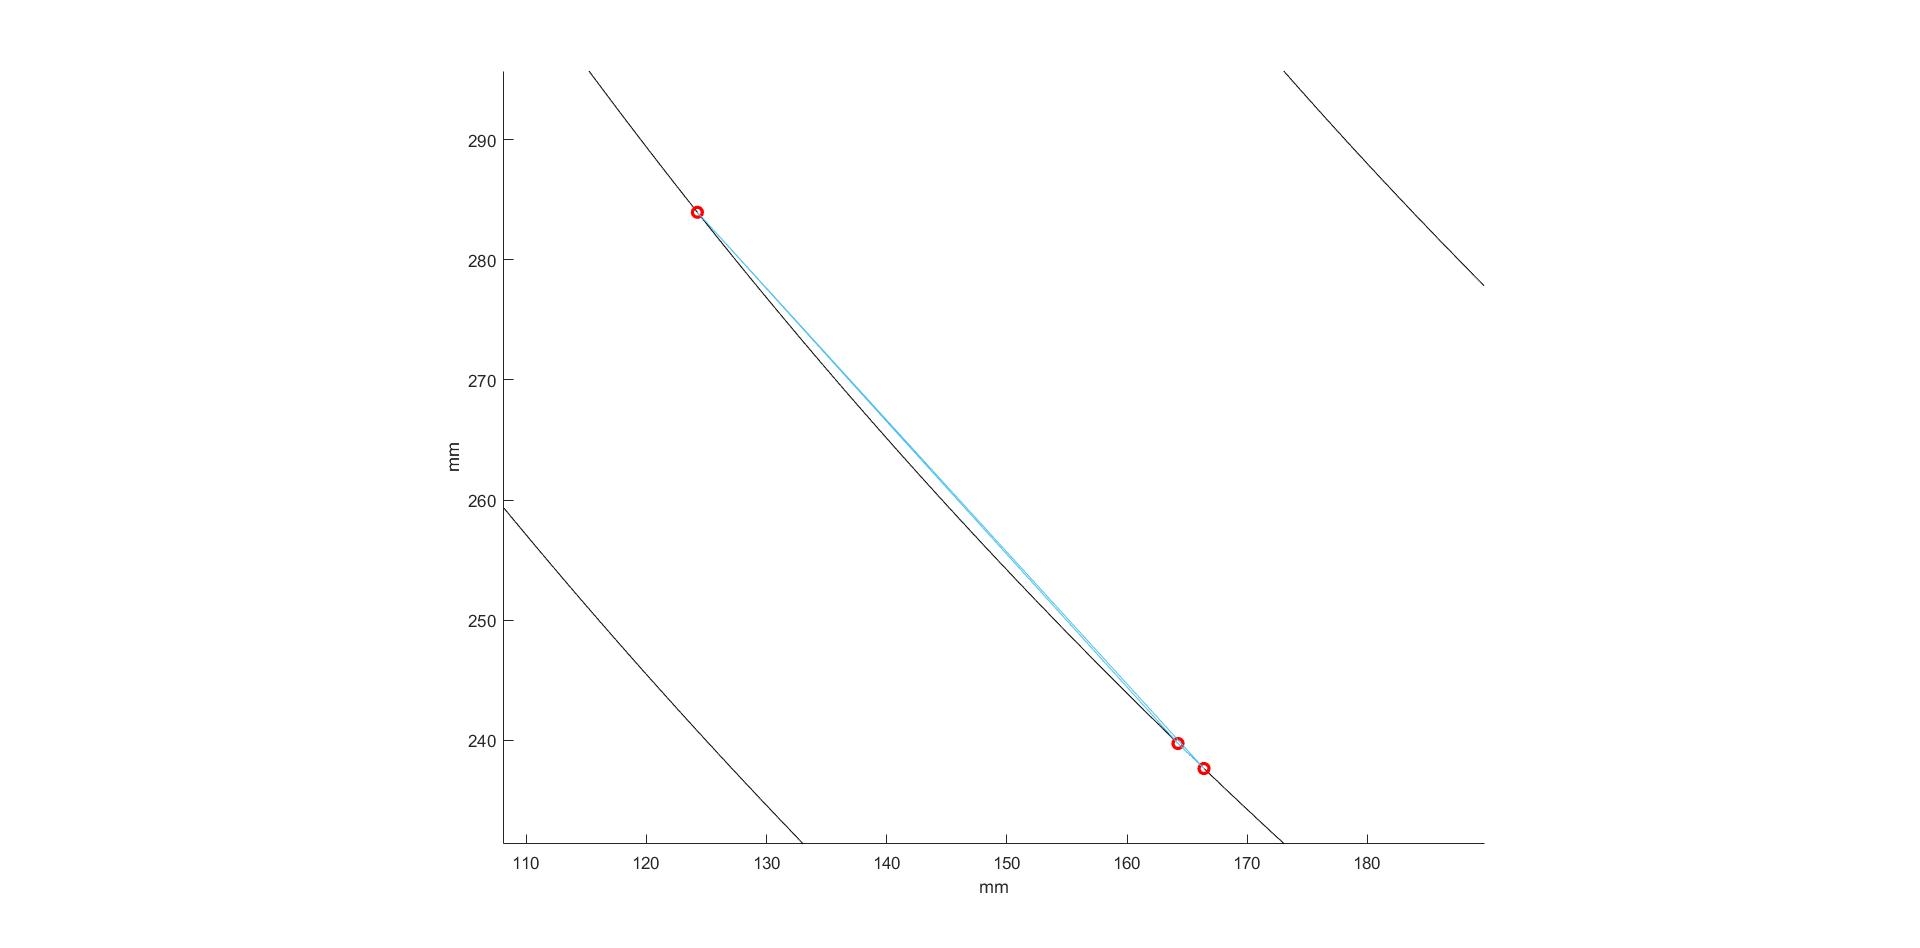
\includegraphics[width=\textwidth]{./images/diameter/c1_worst.jpg}
    \end{minipage}
    
    \caption{Better (on the top) and worst (on the bottom) scenarios, accordingly with the error distribution.}
    \label{fig:diam:scenarios}
  \end{figure}
\clearpage %%%%%%%%%%%%%%%%%%%%%%%%%%%%%%%%%%%%%%%%%%%%%%%%%%%%%%%%%%%%%%%%%%%%%%%%%%%%%%%%%%
  \begin{figure}[t!]
    \centering
    \begin{minipage}[c]{0.9\textwidth}
      \centering
      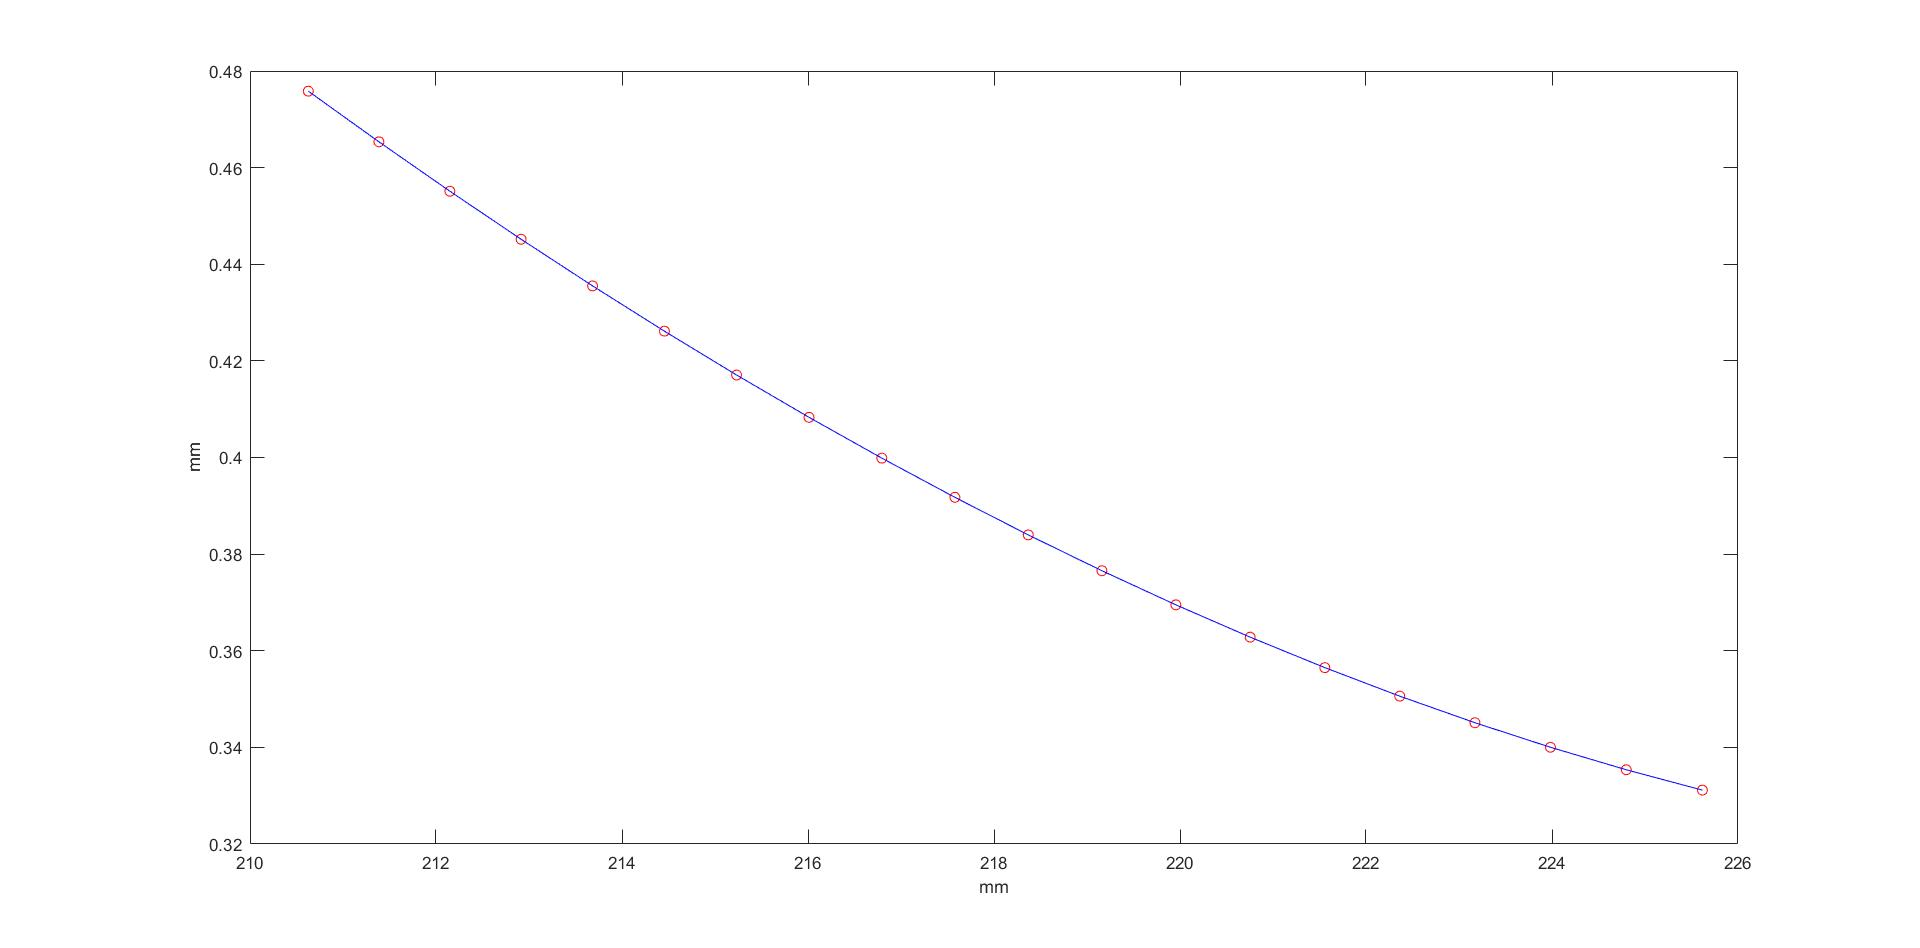
\includegraphics[width=\textwidth]{./images/diameter/H1_1.jpg}
    \end{minipage}
    \vfill
    \begin{minipage}[c]{0.9\textwidth}
      \centering
      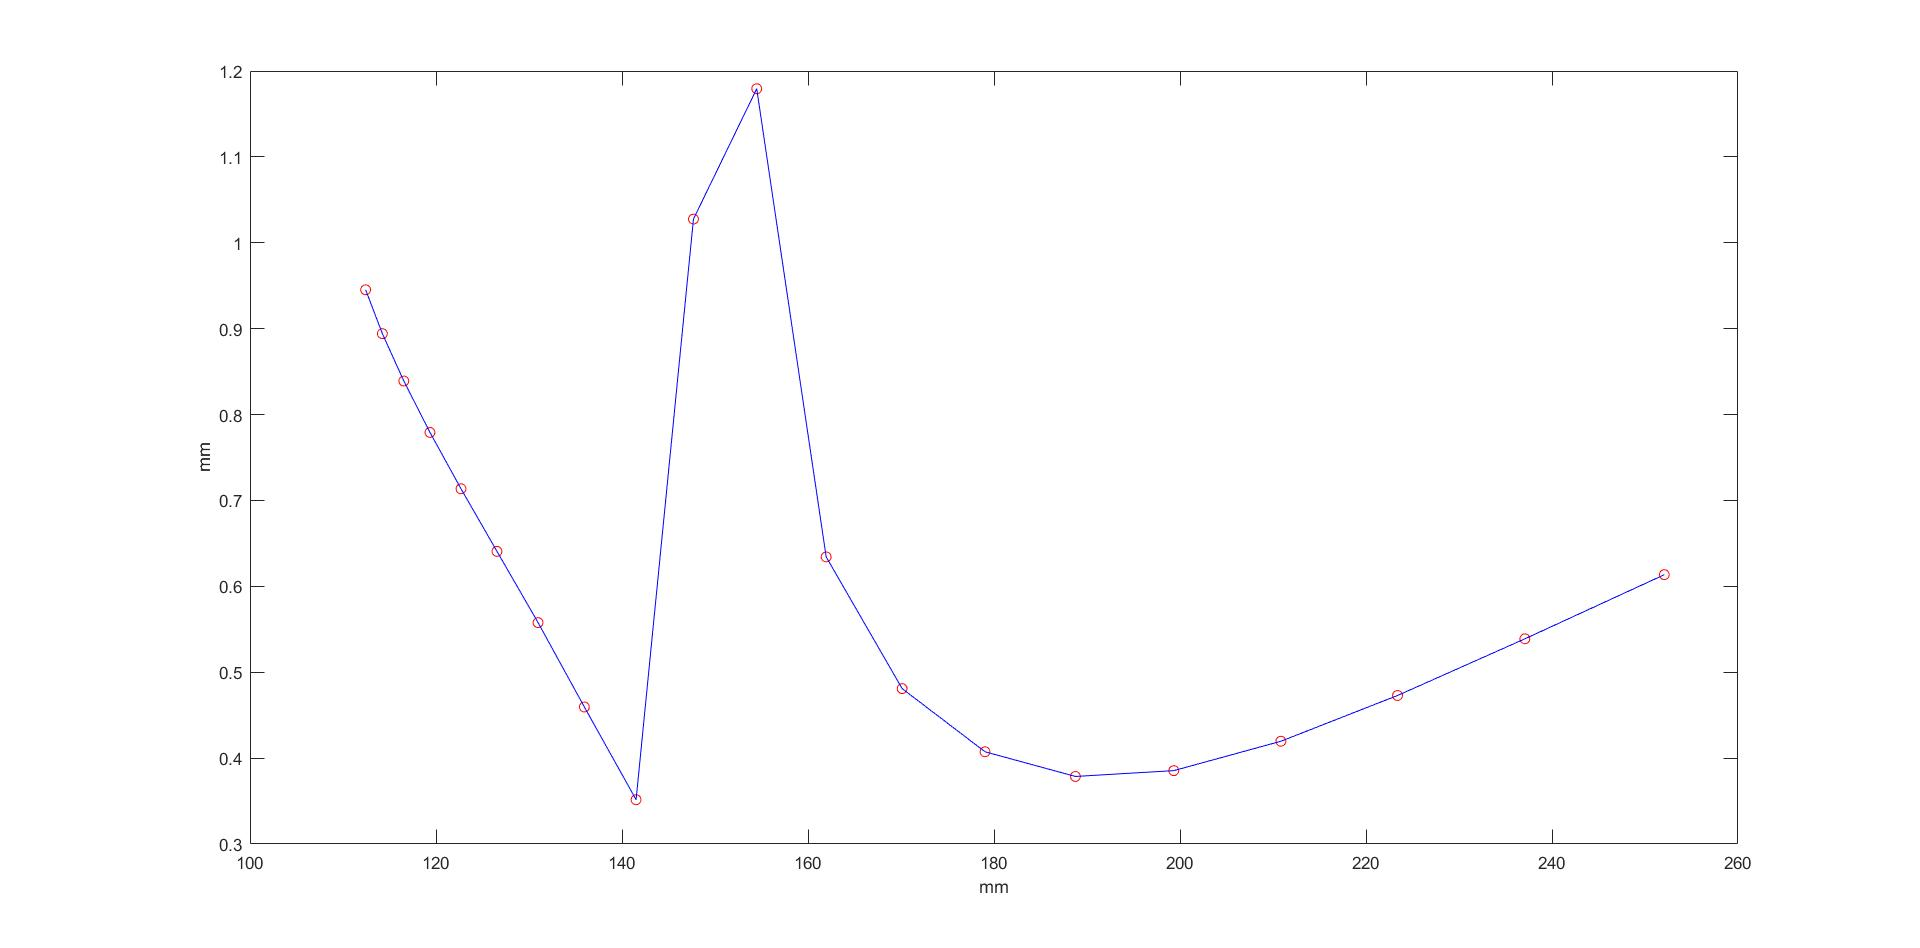
\includegraphics[width=\textwidth]{./images/diameter/H2_1.jpg}
    \end{minipage}
    
    \caption{Error distributions as the position of the first laser projector (top) and the second (bottom).}
    \label{fig:diam:hs}
  \end{figure}
  \begin{table}[h!]
  \small
  \centering
  \begin{tabular}{|r|r|r|r|r|r|r|r|r|}
  \hline
  \multicolumn{1}{|c|}{\textbf{Error}} & \multicolumn{1}{c|}{\textbf{$Y_1$}} & \multicolumn{1}{c|}{\textbf{$Y_2$}} & \multicolumn{1}{c|}{\textbf{$Y_3$}} & \multicolumn{1}{c|}{\textbf{$L_1$}} & \multicolumn{1}{c|}{\textbf{$L_2$}} & \multicolumn{1}{c|}{\textbf{$L_3$}} & \multicolumn{1}{c|}{\textbf{P}} & \multicolumn{1}{c|}{\textbf{A}} \\ \hline
  \multicolumn{1}{|c|}{\textit{(mm)}}  & \multicolumn{1}{c|}{\textit{(mm)}}  & \multicolumn{1}{c|}{\textit{(mm)}}  & \multicolumn{1}{c|}{\textit{(mm)}}  & \multicolumn{1}{c|}{\textit{(mm)}}  & \multicolumn{1}{c|}{\textit{(mm)}}  & \multicolumn{1}{c|}{\textit{(mm)}}  & \multicolumn{1}{c|}{\textit{(mm)}}      & \multicolumn{1}{c|}{\textit{(mm)}} \\ \hline
  0.72	& 225.62	& 170.56	& 150.22	& 59.79	& 44.87	& 98.45	& 203.12	& 864.18	\\ \hline
  0.64	& 223.98	& 170.56	& 150.22	& 57.50	& 44.87	& 95.88	& 198.25	& 852.46	\\ \hline
  0.58	& 222.36	& 170.56	& 150.22	& 55.24	& 44.87	& 93.31	& 193.43	& 841.07	\\ \hline
  0.53	& 220.75	& 170.56	& 150.22	& 53.03	& 44.87	& 90.75	& 188.66	& 830.03	\\ \hline
  0.49	& 219.16	& 170.56	& 150.22	& 50.87	& 44.87	& 88.21	& 183.95	& 819.33	\\ \hline
  0.48	& 217.58	& 170.56	& 150.22	& 48.77	& 44.87	& 85.67	& 179.31	& 808.96	\\ \hline
  0.49	& 216.01	& 170.56	& 150.22	& 46.73	& 44.87	& 83.14	& 174.74	& 798.94	\\ \hline
  0.53	& 214.46	& 170.56	& 150.22	& 44.76	& 44.87	& 80.63	& 170.26	& 789.26	\\ \hline
  0.58	& 212.91	& 170.56	& 150.22	& 42.87	& 44.87	& 78.13	& 165.87	& 779.92	\\ \hline
  0.66	& 211.39	& 170.56	& 150.22	& 41.08	& 44.87	& 75.64	& 161.59	& 770.92	\\ \hline
  \end{tabular}
  \caption{Example of committed error, while estimating the diameter}
  \label{tab:diam:tab1}
\end{table}

\clearpage
\noindent
remarkable result was found. \\

To conclude this first part of the analysis, we can say that an at least quadratic relation exists between the error made using Erone's formula and the reciprocal distances between the points involved by the measure. Nevertheless, the number of factors that influenced this measures, is big enough to make tricky the definition of a mathematical relation among the involved components. From our point of view, this could be modelled as a linear programming minimum search problem. \\

As we can realize from the analysis above, we were not interested in the numerical results, but only in the distribution of the error over the position of the points. In fact, in the case of study we knew the performance of the model in real scenarios. However, the results in our possession did not take into account the error due to $y_i$'s estimates. So we performed a last set of test to introduce this last factor.

\subsection{Error propagation} %%%%%%%%%%%%%%%%%%%%%%%%%%%%%%%%%%%%%%%%%%%%%%%%%%%%%%%%%%%
To conclude our analysis on this last part of the model, we correctly set al the parameters with typical values, that we had seen work properly for our systems. The empirical data that we initially used to study the problems, the \textit{bad calibrated ones}, where obtained using a device like the one described in Section \ref{sec:exp2}, so the values used for estimate $\sigma_{y_i}$ was the ones shown in Table \ref{tab:exp2:refereces}. 
As we said in the previous subsection, we didn't find a useful relation between the error and the input parameters, so they are too much to synthesize the results in a simple table. Furthermore, as we shown in the figures above, there wasn't a distribution for witch the data could take sense. In Table \ref{tab:diam:tab1} we reported an example of data, collected keeping fix the system, and moving the wheel along the rails. In this case, as well as in the others, we noticed that the $\sigma_{y_i}$ did not heavily affect the final error of the measure, which always remains within the range $\left(0.1, \, 1.0\right) \, mm$. The cases where the error became greater, were in limit working condition for the system, such with the wheel over the projector. The $Y_i$ columns are the lengths of the simulated $y_i$ vectors, while the $L_i$ columns are the lengths of the sides of the triangle inscribed in the circumference; $P$ and $A$ are the perimeter and the area, respectively. Furthermore, we preferred not to return the diameter of the wheel, because the wheel being simulated, and this value was always perfectly accurate.

%